\begin{frame}
    \frametitle{Why Generation IV Reactors?}
    \begin{itemize}
      \item Energy use and production contribute two-thirds of total \gls{GHG} emissions \cite{noauthor_climate_2018}
      \item Because energy generation technology selection profoundly impacts climate change, 
      large scale emissions-free nuclear power deployment could 
      significantly reduce GHG production but faces both cost and perceived adverse 
      safety challenges \cite{noauthor_climate_2018, petti_future_2018}.
      \item The Generation IV International Forum identified six Generation IV systems 
      that target goals in four areas: sustainability, 
      economics, safety and reliability, and proliferation resistance and physical 
      protection: GFR, LFR, MSR, SFR, SCWR, and VHTR. 
      \begin{figure}[htbp!]
          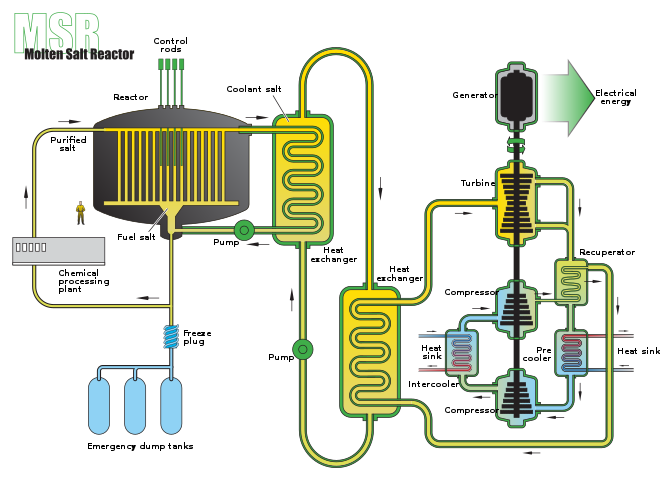
\includegraphics[height=2.8cm]{figures/msr}
          \hspace{1cm}
          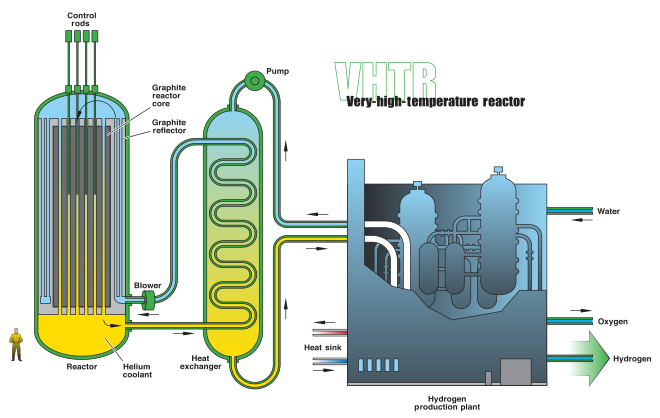
\includegraphics[height=2.8cm]{figures/vhtr}
      \end{figure}
    \end{itemize}
  \end{frame}
\begin{frame}
  \frametitle{MSRs and VHTRs}
  \begin{block}{Molten Salt Reactor (MSR) System}
    \begin{itemize}
      \item Produces fission power in circulating molten salt fuel mixture
      \item Molten Fluoride Salts have have chemical stability, low vapor pressure 
      at high temperatures, good heat transfer properties, resistance against 
      radiation damage, and inert to common structural materials
      \item Inherent system safety with fail-safe drainage, passive cooling, and 
      low inventory of volatile fission products in the fuel
    \end{itemize}
  \end{block}
  \vspace{-0.25cm}
  \begin{block}{Very High Temperature Reactor System (VHTR)}
    \begin{itemize}
      \item Tristructural Isotropic (TRISO) fuel withstands high burnup and 
      temperature
      \item High outlet temperature increases power conversion efficiency, reduces 
      waste heat generation, and enables high-temperature heat applications 
      such as hydrogen production
      \item Helium coolant's high 100 atm pressurization requires an expensive thick
      concrete reactor vessel
    \end{itemize}
  \end{block}
\end{frame}
\begin{frame}
  \frametitle{FHR}
  \begin{itemize}
    \item \acrlong{FHR} concept combines the best aspects of \acrlong{MSR} and \acrlong{VHTR} technologies. 
      \acrshort{FHR} use high-temperature coated-particle fuel (similar to the \acrshortpl{VHTR}) 
      and a low-pressure liquid fluoride-salt coolant (similar to the \acrshortpl{MSR})
      \cite{forsberg_fluoride-salt-cooled_2012,facilitators_fluoride-salt-cooled_2013}.
  \end{itemize}
  \begin{block}{\acrfull{FHR} Benefits}
    \begin{itemize}
      \item FHR system has low operating pressure, thus does not require thick 
      concrete pressure vessel 
      \item Molten salt coolant has superior cooling and moderating properties 
      compared to helium coolant in VHTRs
      \item FHR system has large thermal margin enabled by molten salt coolant
      \item FHRs' TRISO particles' solid fuel cladding adds an extra barrier to 
      fission product release compared to MSRs with liquid fuel.
    \end{itemize}
  \end{block}
\end{frame}
\begin{frame}
  \frametitle{AHTR}
  \begin{block}{Advanced High Temperature Reactor Design}
    \begin{itemize}
      \item Design developed by Oak Ridge National Laboratory (ORNL)
      \item Prismatic FHR design with 252 hexagonal fuel assemblies consisting of 
      18 fuel planks arranged in 3 diamond-shaped sectors. 
    \end{itemize}
  \end{block}
  \begin{figure}[]
    \centering
    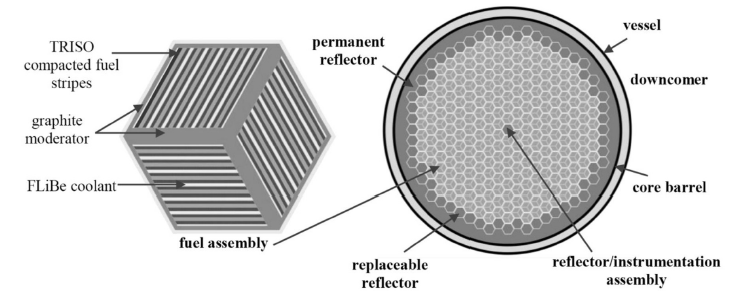
\includegraphics[width=0.8\linewidth]{../docs/figures/ahtr.png} 
    \caption{\acrlong{AHTR} fuel assembly (left) and core configuration (right) 
    reproduced from \cite{ramey_monte_2018}.}
    \label{fig:ahtr}
\end{figure}
\end{frame}

\begin{frame}
  \frametitle{AHTR Geometry}
  \begin{block}{Advanced High Temperature Reactor Design}
    \begin{itemize}
      \item Each fuel plank contains 2 fuel stripes that consists of a cubic 
      lattice of TRISO fuel particles
    \end{itemize}
  \end{block}
  \vspace{-0.3cm}
  \begin{figure}[]
    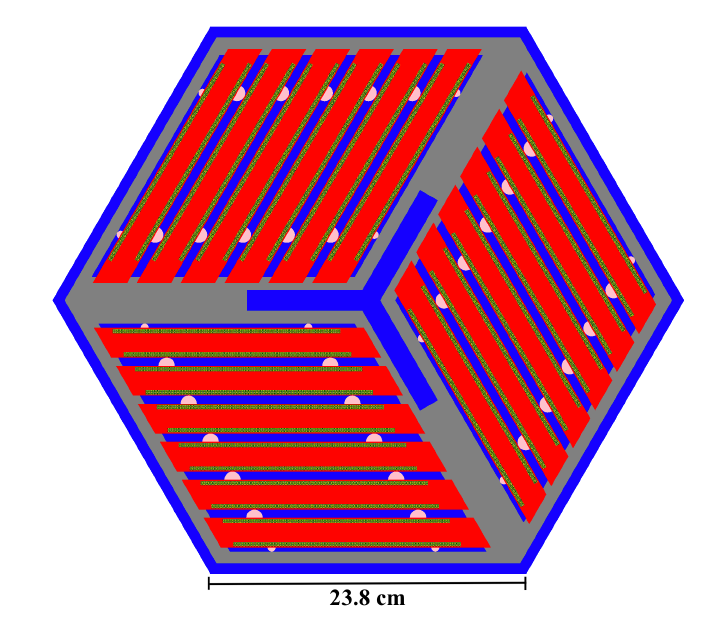
\includegraphics[width=0.45\linewidth]{figures/ahtr-assembly.png} 
    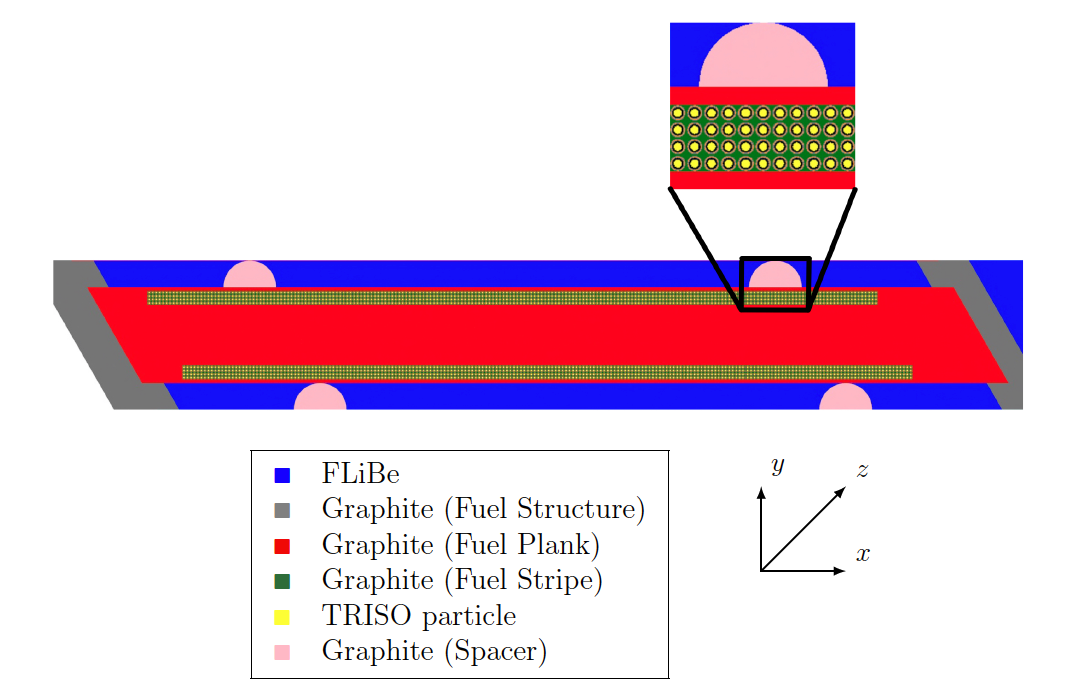
\includegraphics[width=0.45\linewidth]{figures/ahtr-plank.png} 
    \caption{\acrfull{AHTR} fuel assembly with 18 fuel plates arranged in 
    three diamond-shaped sectors, with a central Y-shaped and external channel 
    graphite structure.}
\end{figure}
\end{frame}

\begin{frame}
  \frametitle{FHR Benchmark}
  \begin{itemize}
    \item The AHTR's fuel geometry has triple heterogeneity resulting in
    complex reactor physics and significant modeling challenges
    \item To address and further understand the technical challenges for 
    AHTR modeling, in 2019 the OECD-NEA initiated a FHR benchmark exercise. Its objective 
    is to identify the applicability, accuracy, and practicality of the latest 
    methods and codes to assess the current state of the art of FHR simulation 
    and modeling. The benchmark also enables the cross-verification of software 
    and methods for the challenging AHTR geometry, which is especially useful 
    since applicable reactor physics experiments for code validation are scarce
  \end{itemize}
  \begin{figure}[]
    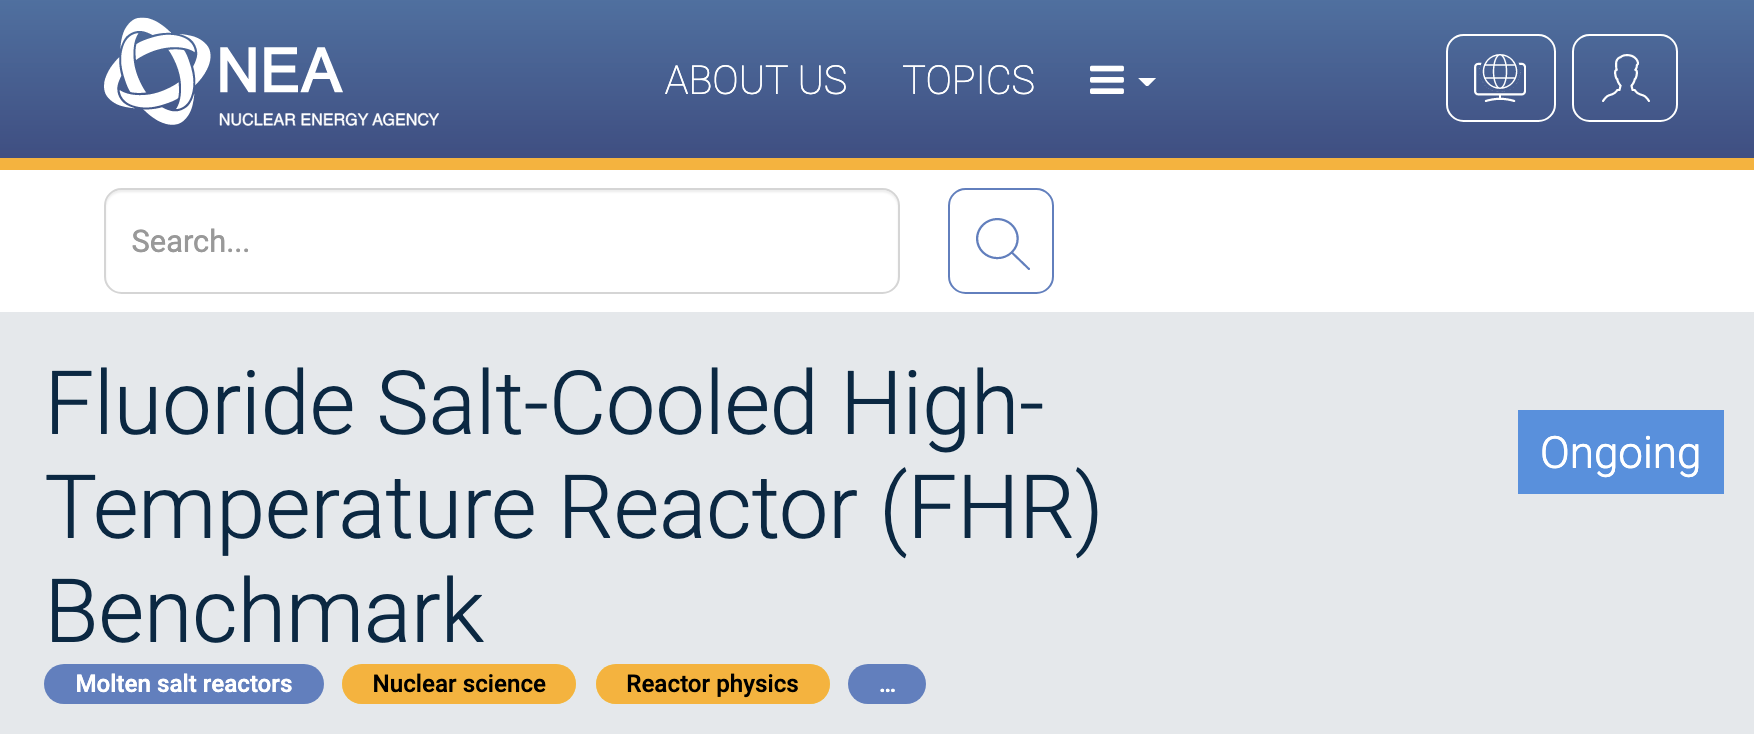
\includegraphics[width=0.5\linewidth]{figures/benchmark.png} 
    \caption{OECD NEA's FHR Benchmark \cite{petrovic_benchmark_2021}.}
\end{figure}
\end{frame}
